% chercher des documents LaTeX dans styles, corps et bib
\makeatletter\def\input@path{{styles/}{corps/}{bib/}}\makeatother

\documentclass[12pt, openany]{report}
\usepackage[a4paper,vdivide={*,22cm,4cm}]{geometry}
\usepackage[french]{babel}
\selectlanguage{french}
\usepackage[T1]{fontenc}
\usepackage[utf8]{inputenc}
\usepackage{pageGardeEnsta}
\usepackage{lmodern}
\usepackage{enumitem}
\usepackage{subcaption}
\usepackage{wrapfig}
\usepackage[colorlinks = true,
            linkcolor = blue,
            urlcolor  = blue,
            citecolor = blue,
            anchorcolor = blue]{hyperref}
% pour charger des images
\usepackage{graphicx}
% répertoire dans lequel trouver les images
\graphicspath{{imgs/}}
% liens hypertexte dans le document
\usepackage[colorlinks,breaklinks]{hyperref}
\setlength{\parindent}{0pt}
\usepackage{float}
\usepackage{hyperref}
\usepackage{listings}
\usepackage[round]{natbib}
\usepackage{appendix}

\title{Simulation d'un robot \\ --Warthog--}
\author{Colin Baumgard, Ludovic Diguet, Hamid Hacene, Corentin Lemoine, Antonin Lizé}
\date{\today}
\doctype{Simulation des robots mobiles}
\promo{UE 4.2}
\etablissement{\textsc{Ensta} Bretagne\\2, rue François Verny\\
  29806 \textsc{Brest} cedex\\\textsc{France}\\Tel +33 (0)2 98 34 88 00\\ \url{www.ensta-bretagne.fr}}
\logoEcole{
\includegraphics[height=4.2cm]{logo_ENSTA_Bretagne_Vertical_CMJN}}
\imgGarde{\centering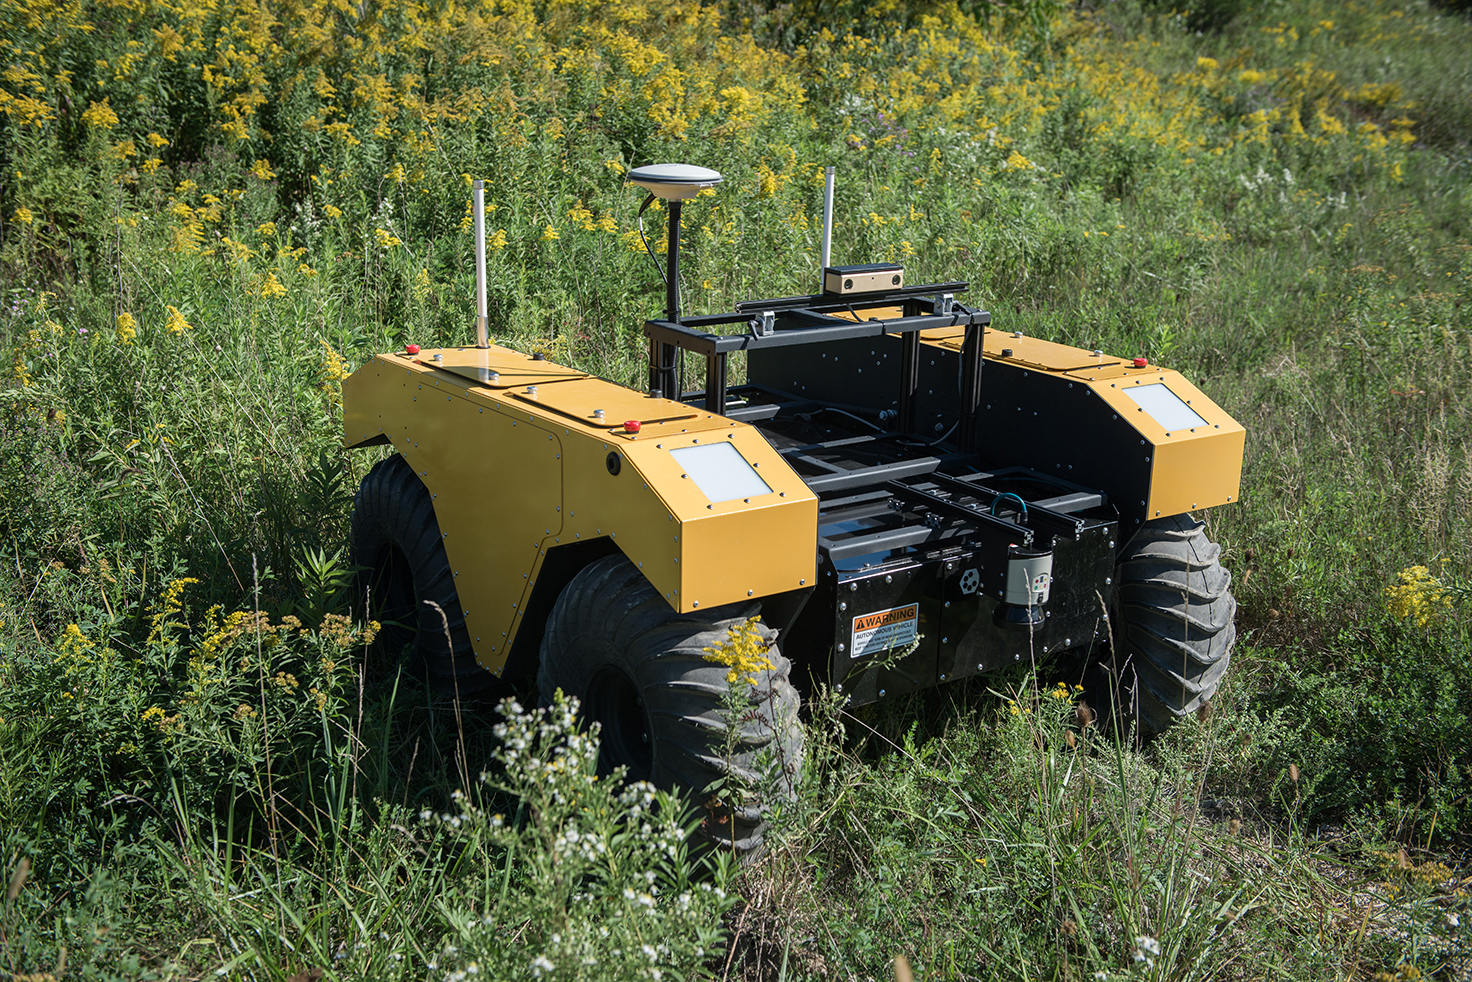
\includegraphics[scale=0.2]{Warthog_UGV-3_1.jpg}}

\renewcommand{\thesection}{\arabic{section}}
\begin{document}
\maketitle
\tableofcontents

\section*{Introduction} 
\addcontentsline{toc}{chapter}{Introduction}
Ce projet s'inscrit dans le cadre des enseignements de l'\textsc{ENSTA Bretagne} dispensés aux élèves de deuxième année de la filière \textit{Robotique Autonome} au sein de l'U.E 4.2 : \textit{Simulation des Robots Mobiles}.\\

Ce rapport présente le travail de notre équipe sur la simulation sur \textit{V-REP} d'un robot : le robot \textit{Warthog} fraîchement acheté par l'\textsc{ENSTA Bretagne}.
Dans la suite du projet nous allons aborder différents aspects de la simulation : le choix de la modélisation des liaisons du robot, le choix de la répartition des masses, le franchissement d'obstacles qui est l'une des caractéristiques principale de ce robot et enfin son comportement et sa simulation dans l'eau.

\section{Modélisation du robot}
\subsection{Choix techniques}
Après avoir étudier la documentation présente sur internet à propos du robot \textit{Warthog} et après visualisation de quelques vidéos, nous avons opté pour la modélisation dynamique suivante :

\begin{itemize}[label=\textbullet, font=\small]
    \item Les 4 roues seront modélisées avec 4 cylindres ;
    \item Les deux trains ainsi que le châssis principal seront modélisés par des parallélépipèdes ;
    \item Pour modéliser les actionneurs des roues, nous utiliserons 4 liaisons pivots simples ; 
    \item La modélisation des deux articulation "bascules" est détaillée plus bas. \ref{sec:bascules}
\end{itemize}

\begin{figure}[H]
     \centering
     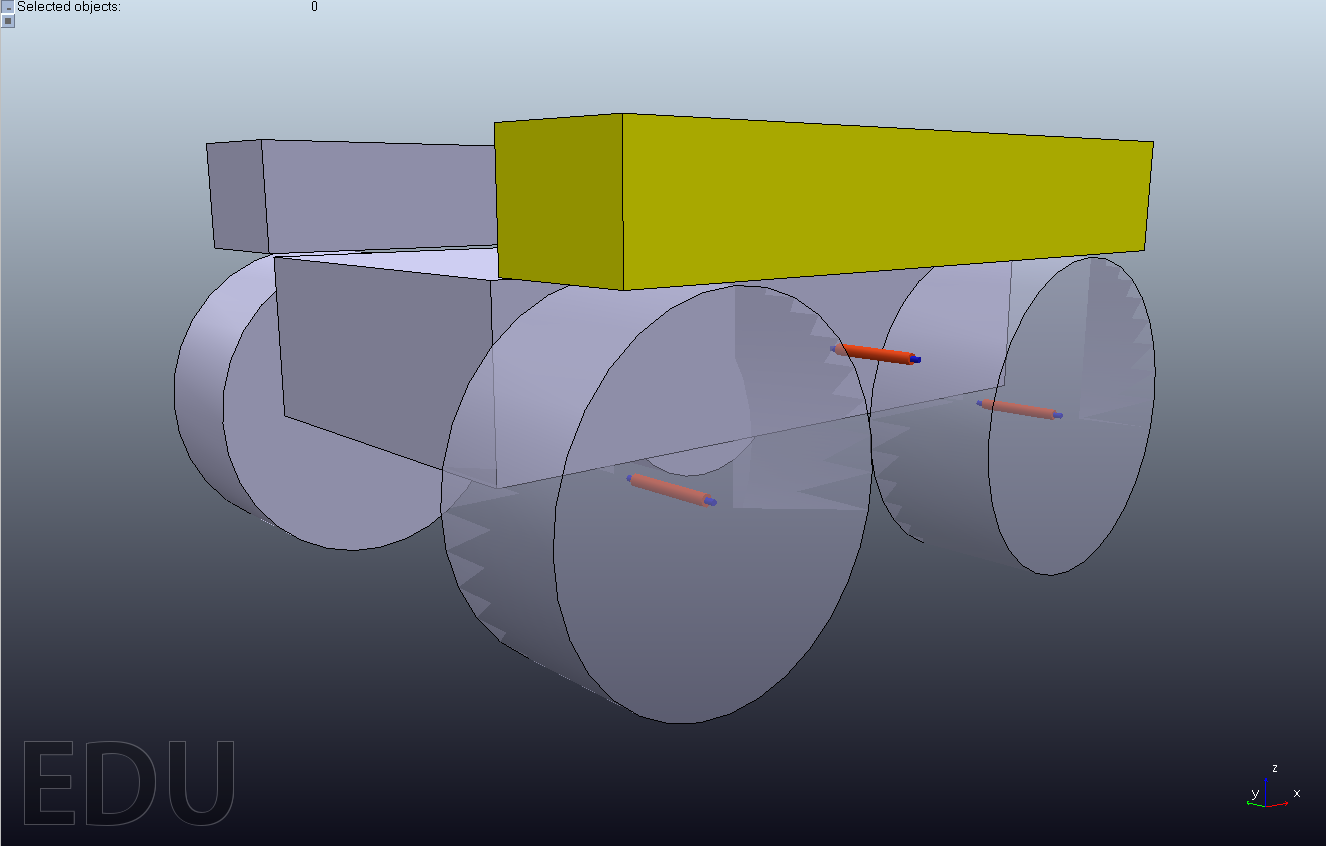
\includegraphics[width=8cm, height=6cm]{sim_dyn.png}
     \caption{Modèle dynamique}
     \label{fig:mdyn}
\end{figure}

\subsection{Répartition du poids}
Dans cette partie nous allons aborder notre choix de répartition de la masse. En effet dans la documentation disponible sur le site du fournisseur, le robot a une masse de 250kg. Nous avons décidé la répartition suivante :
\begin{figure}[H]
     \centering
     \includegraphics[width=10cm, height=7cm]{Répartition_masse.png}
     \caption{Répartition des masses}
     \label{fig:masse}     
\end{figure}

\subsection{Articulations des deux "bascules" portes roues}
\label{sec:bascules}
\begin{wrapfigure}{r}{0.5\textwidth}
    \begin{center}
        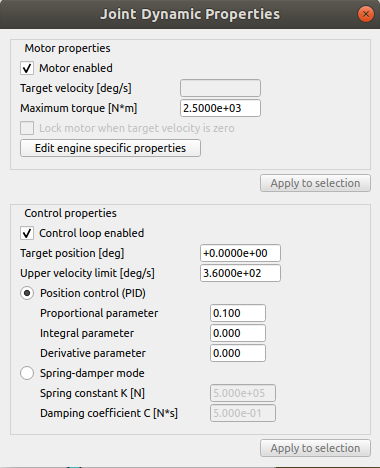
\includegraphics[width=5cm, height=7cm]{joint.png}
    \end{center}
    \caption{Propriétés de l'articulation}
    \label{fig:joint}     
\end{wrapfigure}

Dans un premier temps, nous avons modélisé cette articulation avec une liaison pivot en mode \textit{Spring-damper mode}. Après plusieurs tests pour régler les deux coefficients $k$ et $C$, le comportement de notre robot ne se rapprochait pas de ce que nous avons pu voir sur les vidéos de présentation du \textit{Warthog}.\\

Nous avons donc décidé de changer d'approche. Le comportement de cette liaison pivot dans les vidéos montre qu'elle agit comme un vérin : elle essaie de maintenir le plus possible le châssis principal à l'horizontale. Quand l'environnement ne le permet pas (passage sur une roche par exemple), la liaison ramène progressivement le châssis à sa position d'équilibre.\\

Nous avons donc décidé de la modéliser par une liaison pivot simple avec les propriétés de la figure \ref{fig:joint}. En effet, un contrôleur \textit{PD} se comporte comme un système ressort-amortisseur : il ramène notre système à la position d'équilibre. 

\subsection{Interface avec \textsc{ROS}}
Pour communiquer et pouvoir tester le robot et sa modélisation, nous avons établi une interface avec \textsc{ROS} en \textit{lua}. Cette interface permet de contrôler les quatre moteurs de notre robot.
\begin{figure}[H]
     \centering
     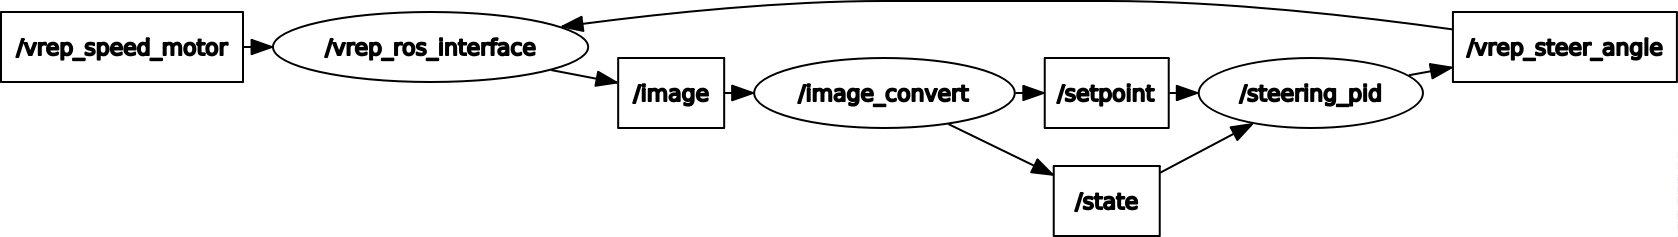
\includegraphics[width=\textwidth, height=4cm]{rosgraph.png}
     \caption{Interface \textsc{ROS}}
     \label{fig:rosgraph}     
\end{figure}

\subsection{Validation du modèle}
Afin de valider le modèle dynamique, nous avons construit une scène avec différents obstacles. Un script \textit{python} est utilisé pour contrôler le robot avec les touches du clavier. Cette utilisation nous a permis de valider les différentes valeurs des coefficients du \textit{PID}.\\

Une vidéo de la simulation en fonctionnement est diponible à cette \href{https://youtu.be/z00VfYflSLs}{adresse}\footnote{https://youtu.be/z00VfYflSLs}. Les nodes nécessaires pour contrôler le robot avec le clavier sont \textit{kb\_t} du package \textit{keyboard\_transcript} ainsi que \textit{key\_teleop} du package éponyme. 

\begin{figure}[H]
     \centering
     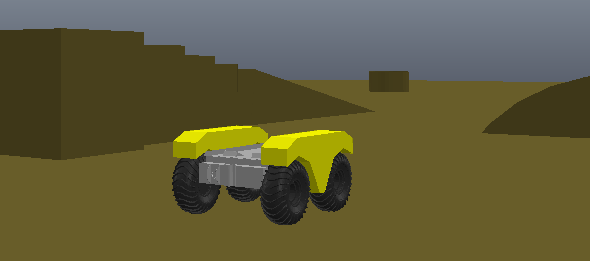
\includegraphics[scale=0.5]{resu.png}     
     \caption{Simulation et validation}
     \label{fig:resu}
\end{figure}


\section{Simulation du robot dans l'eau}


\subsection{Simulation d'une simple sphère}
Afin de mettre en place une simulation simplifiée comme preuve de faisabilité, nous avons cherché à simuler une sphère dans l'eau.\\

\begin{figure}[H]
     \centering
     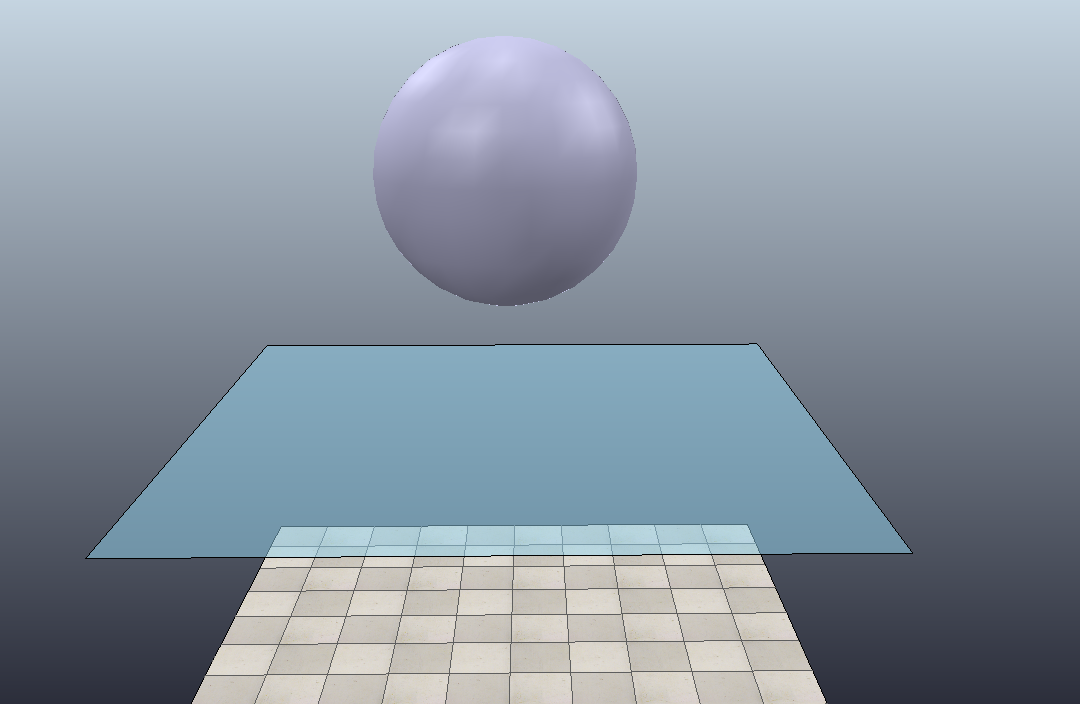
\includegraphics[width=10cm]{scene sphere.png}     
     \caption{Scène V-rep de la sphère au dessus d'un volume d'eau}
     \label{fig:resu}
\end{figure}
Dans la figure ci-dessus, on voit la scène V-rep. Un script en lua fait ensuite le lien avec un node ROS codé en C++. Pour simuler l'action de l'eau sur la sphère, le script récupère la position de celle-ci. Un calcul de la poussée d'Archimède est ensuite effectué. On a besoin pour cela de la formule de la calotte sphérique, énoncé ci-dessous : 

\begin{figure}[H]
     \centering
     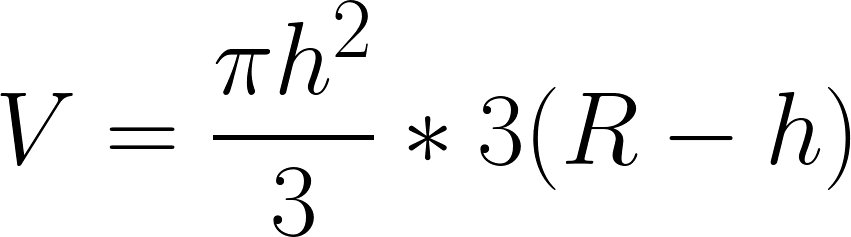
\includegraphics[width=4cm]{form_cal_sph.png}
\end{figure}
Avec h la hauteur immergé et R le rayon de la sphère. On en définit ensuite facilement la poussée d'Archimède, que l'on applique au centre de la sphère (la force s'applique au fait au barycentre du volume immergé, mais comme celle-ci est coaxiale et passant par le centre de gravité, cette hypothèse est vérifiée puisqu'aucun moment n'est créé). Il ne reste alors qu'à renvoyer la valeur de cette force au script lua qui l'applique dans V-rep.\\

Nous obtenons alors une balle rebondissante. Il faut, pour une simulation plus réaliste, intégrer un coefficient de frottement. Pour cela, le code lua transmettra en plus de la position, la vitesse. Une première approche a été de calculer la vitesse en dérivant la position, mais le résultat est moins propre qu'avec la vitesse extraite de V-rep, qui est donc ajoutée aux topics. Pour le coefficient de frottement, nous avons choisi un frottement linéaire et quadratique.\\

Nous obtenons un résultat tout à fait conforme à nos attentes. Une petite tricherie est toutefois nécessaire pour éviter la divergence de la simulation. On place une liaison glissière entre le sol et la sphère, en ne lui autorisant que la translation selon z, hypothèse vérifiée par la symétrie selon cet axe.

\subsection{Application au robot Warthog}
Pour la simulation du robot complet dans l'eau, nous avons implémenté la méthode qui consiste à appliquer une force sur chaque roue égale à la force d'Archimède résultante de leur partie immergée. Cette méthode fonctionne mais le résultat obtenu n'est pas le bon puisque le robot se retourne. Ce comportement est la conséquence du placement des points d'application des forces vis-à-vis du centre de gravité du robot. L'équilibre instable initial est perturbé par des erreurs de calculs liées à la simulation et le robot atteint un équilibre stable sur le dos.\\

Le meilleur moyen de corriger ces erreurs serait de faire des calculs de stabilité pour trouver le moment du couple de redressement ainsi que la poussée d'Archimède pour une grande plage d'attitudes du robot, et d'utiliser ces calculs dans des \textit{Look Up Tables} pour notre simulation.

\section*{Conclusion}
\addcontentsline{toc}{chapter}{Conclusion}
Pour conclure, ce projet nous a permis de mettre en pratique les premiers cours d'utilisation de \textit{V-REP}. En associant ces connaissances ainsi que l'utilisation de ROS pour contrôler le robot pendant le simulation, nous avons réussi à modéliser simplement et rapidement un robot dans une situation donnée \textit{(évitement d'obstacles, navigation dans l'eau)}.

\listoffigures
\end{document}
